\documentclass[12pt, a4paper]{article}
%=========================== PACKAGES =============================%

\usepackage[utf8]{inputenc} 
\DeclareUnicodeCharacter{00A0}{ }

\usepackage[hmargin=1.5cm,vmargin=1.5cm]{geometry}
\usepackage[brazil]{babel}

\usepackage{longtable}
  
\usepackage{graphicx}
\usepackage{placeins}
\usepackage{subcaption}
\usepackage{float} 

\usepackage{hhline}
\usepackage{courier}
 
\usepackage{amsmath}
\usepackage{bm}
\usepackage{amsfonts}

\usepackage{hyperref}

\usepackage{listings}
\renewcommand\lstlistingname{Programa}
 
 
\usepackage{color} %red, green, blue, yellow, cyan, magenta, black, white
\lstset{language=bash,%
    basicstyle=\footnotesize\ttfamily,
    breaklines=true,%
    keywordstyle=[4]{\color{black}},
    frame= single,
}
 
\lstdefinestyle{nonumbers}
{numbers=none} 

\usepackage{multirow}


\usepackage{float}

\usepackage{enumerate}

%=========================== PACKAGES =============================%


\author{Gustavo Ciotto Pinton}

\begin{document}

\begin{titlepage}
\vspace*{.28\textheight}
\begin{center}
%
\begin{figure}[h]
    \centering
    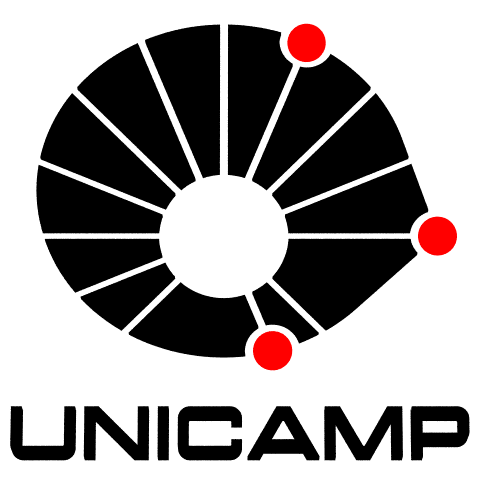
\includegraphics[scale=0.18]{image/LogoUnicamp}
\end{figure} 
%
\vspace*{10pt}
%\text{ }\\[7 cm]
\textbf{\LARGE Exercício de Fixação de Conceitos 2} \\ \vspace{12pt}
\textbf{\large EA072 - Inteligência Artificial em Aplicações Industriais}
\vspace*{72pt}

Gustavo \textbf{CIOTTO PINTON} - \textbf{RA 117136}
 

Campinas, \today

\end{center}
\end{titlepage}

\newpage

\tableofcontents

\newpage

\section {\textit{Netwok Time Protocol} - NTPv4}

\subsection {Introdução}

O protocolo NTP implementa diversas soluções que permitem a sincronização dos
relógios dos computadores pertencentes a uma determinada rede. O protocolo
utiliza diversas métricas, descritas nas próximas seções, a fim de determinar
quais são as fontes mais seguras e consistentes para obter a melhor
sincronização e uma maior precisão. Somadas a essas estatísticas, o NTP faz uso
de algoritmos de seleção, \textit{cluster} e combinação que garantem, por sua
vez, a determinação dos servidores mais confiáveis a partir de um número finito
de amostras provindas de tais fontes. 

\vspace{12pt}

A troca de mensagens é feita através de pacotes UDP, sendo que o protocolo
suporta tanto o IPv4 quanto o IPv6. Apesar do fato de que o protocolo UDP não
oferece garantias de entrega e correção de eventuais erros ou duplicatas, o
NTPv4 implementa mecanismos, tais como o \textit{On-Wire protocol}, capazes de
verificar a consistência dos dados contidos nos pacotes recebidos e, assim,
agir corretamente em casos de perdas ou pacotes repetidos.

\vspace{12pt}

Neste relatório, serão discutidas as características da versão 4 do NTP,
especificadas no RFC5905. Esta versão aprimora alguns aspectos da versão 3
(NTPv3) e adiciona algumas outras funcionalidades, como, por exemplo, a
descoberta dinâmica de servidores (\textit{automatic server discovery}),
sincronização rápida na inicialização da rede ou depois de falhas
(\textit{burst mode}) e uso da criptografia \textit{Public-key}.

\subsection {Características do Protocolo}

O primeiro aspecto importante do protocolo NTPv4 é a organização dos
nós de uma rede. O NTP provê 3 tipos diferentes de variantes 
e 6 modos de associação, que identificam a função de cada nó que
compõe um comunicação. As variantes NTP são, portanto:

\begin {enumerate}[i.]
  
  \item \textit{server/client}: um cliente envia pacotes a um servidor
  requisitando sincronização, que responde utilizando o endereço contido nos
  respectivos pacotes. Nesta variante, servidores fornecem sincronização aos
  clientes, mas não aceitam sincronizações vindas dos clientes. As associações
  entre os nós nesta variante são persistentes, ou seja, são criadas na
  inicialização do serviço e nunca são destruídas.
  
  \item \textit{symmetric}: neste tipo de variante, um nó se comporta tanto como
  servidor como cliente, isto é, ele recebe e envia informações de sincronização
  ao outro nó. Associações deste tipo podem ser persistentes, conforme explicado
  no item anterior, ou temporárias, isto é, podem ser criadas a partir do
  recebimento de um pacote e eliminadas após um certo intervalo ou ocorrência
  de erro. No primeiro caso, adota-se uma associação \textit{ativa}, enquanto
  que na segunda, adota-se uma \textit{passiva}.
      
  \item \textit{broadcast}: nesta variante, um servidor \textit{broadcast}
  persistente envia pacotes que podem ser recebidos por diversos clientes.
  Quando um cliente recebe um pacote deste tipo, uma associação temporária do
  tipo \textit{broadcast client} é criada e o cliente recebe sincronização até o
  fim de um intervalo ou ocorrência de um erro.
  
\end{enumerate}

O protocolo oferece ainda uma funcionalidade que permite aos clientes
descobrirem servidores disponíveis na rede para sincronização. Tal mecanismo é
chamado de \textit{Dynamic Server Discovery}, que provê dois tipos especiais de
associação: \textit{manycast server} e \textit{manycast client}. Um cliente
\textit{manycast} persistente envia pacotes para endereços de \textit{broadcast}
ou \textit{multicast} e, caso um \textit{manycast server} receba tais pacotes,
ele envia uma resposta a determinado cliente, que, por sua vez, mobiliza uma
associação temporária com o respectivo servidor. A fim de descobrir os
servidores mais próximos, os clientes enviam pacotes com TTL crescentes, até que
o número mínimo de servidores descobertos seja atingido.

\vspace{12pt}

O segundo aspecto importante é a implementação dos processos que são executados
em um sistema a fim de garantir as funcionalidades apresentadas acima. Cada nó
da rede utiliza dois processos dedicados para cada servidor que provê
sincronização, além de 3 outros dedicados para escolha dos melhores candidatos
e ajuste do relógio. A figura \ref{fig:modelo} esquematiza a relação entre tais
processos. As flechas representam trocas de dados entre processos ou algoritmos.
 
\FloatBarrier

\begin{figure}[h]
    
    \centering
    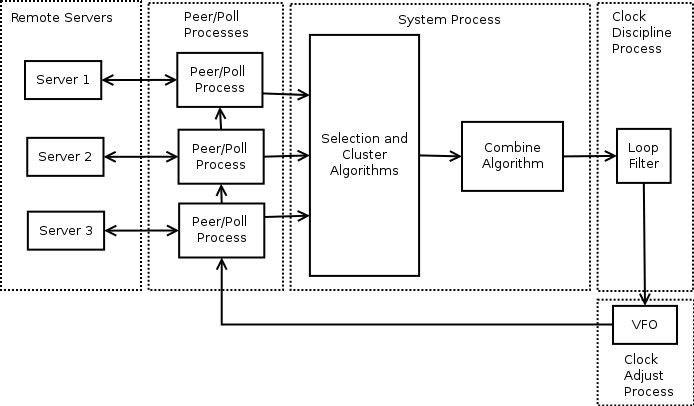
\includegraphics[scale=0.5]{image/ntp_implementation}
    \caption {Implementação dos processos executados por um nó da rede.}
    \label{fig:modelo}
\end{figure} 

\FloatBarrier

Cada componente é, portanto, responsável por uma funcionalidade específica
oferecida pelo NTP. Temos, assim:

\begin {enumerate}[i.]
  \item \textit{Remote servers}: servidores que fornecem sincronização aos nós
  da rede. Tais servidores podem pertencer à mesma rede às quais os clientes
  estão inseridos ou podem ser disponibilizados via Internet por organismos
  responsáveis por gerenciar e garantir que os relógios apresentem tempos
  consistentes. 
  
  A fim de diferenciar os diversos servidores utilizados em relação ao seu grau
  de importância e confiabilidade, o protocolo NTP atribui um nível a cada
  \textit{server}, chamado de \textit{stratum}. Tal atributo vale 1 para
  servidores primários, 2 para servidores secundários e assim sucessivamente. À
  medida que o valor de \textit{stratum} aumenta, a precisão diminui,
  dependendo do estado da rede. O valor máximo deste atributo é 15 e, portanto,
  são permitidos até 15 níveis hierárquicos. O valor 0 é reservado pelo
  protocolo para mensagens de controle e transmissão de estado entre nós. Tais
  mensagens são chamadas de pacotes \textit{Kiss-o'-Death}.
  
%   Caso \textit{stratum} de determinado servidor apresente o valor
%   16, isso significa que o cliente que está tentando obter sincronização está
%   dessincronizado com tal servidor.
  
  \item \textit{Peer/poll processes}: quando um pacote transmitido por um
  servidor chega em um nó, o \textit{peer process} é chamado. Tal processo então
  verifica se o pacote é consistente (\textit{On-Wire protocol}, proteção
  contra perdas e duplicatas) e calcula algumas estatísticas usadas pelos demais
  processos. Tais estatíticas consistem em:
  		
  		\begin{itemize}
  		  \renewcommand\labelitemi{--}
  		  \item \textit{offset} (\(\theta\)): deslocamento de tempo do
  		  relógio do servidor em relação ao relógio do sistema;
  		  \item \textit{delay} (\(\delta\)): tempo que o pacote necessita para
  		  percorrer toda a rede entre cliente e servidor;
  		  \item \textit{dispersion} (\( \epsilon \)): erro máximo inerente à medida
  		  do relógio do sistema;
  		  \item \textit {jitter} (\( \psi \)): raiz do valor quadrático médio dos
  		  \textit{offsets} mais recentes.
  		\end{itemize}
  		
	O \textit{poll process} é responsável, por sua vez, por enviar pacotes aos
	servidores a cada intervalo de \(2^\tau\) segundos. \(\tau\) varia de 4 a 17,
	resultando, assim, em intervalos de 16 segundos a 36 horas. O valor de \(\tau\)
	pode variar durante a execução, sendo modificado pelo algoritmo regulador do
	relógio, que será discutido posteriormente. 
	
	\item \textit{System process}: inclui algoritmos de seleção, clusterização e
	combinação que utilizam as diversas estatísticas obtidas de cada servidor para
	determinar os candidatos mais precisos e confiáveis à sincronização do relógio
	do sistema. As funções de cada algoritmo são, respectivamente:
		
		\begin{itemize}
  		  \renewcommand\labelitemi{--}
  		  \item determinar bons candidatos, isto é, determinar quais servidores
  		  possuem informações de sincronismo efetivamente importantes;
  		  \item determinar os melhores candidatos dentro do conjunto de servidores
  		  julgados importantes no passo anterior;
  		  \item computar estatísticas baseadas nos dados recolhidos dos servidores
  		  presentes no subconjunto escolhido pelo algoritmo de clusterição.
  		\end{itemize}
  	
  	\item \textit{Clock discipline process}: responsável por controlar o tempo e
  	frequência do relógio do sistema;
  	
  	\item \textit{Clock-adjust process}: roda a cada segundo para comunicar aos
  	demais processos os resultados das correções realizadas no relógio do
  	sistema.
  	
\end{enumerate}

\subsection {Exemplo}

A rede representada pela figura \ref{fig:redeNTP} foi proposta a fim de testar o
funcionamento do protocolo NTP. As setas determinam as relações entre os nós e
as direções representam quais nós fornecem e/ou recebem sincronização. Todos os
computadores pertencem à mesma rede, isto é, assume-se que há um \textit{router}
ligando esses nós e responsável pela comunicação com a Internet.

\FloatBarrier

\begin{figure}[h]
    
    \centering
    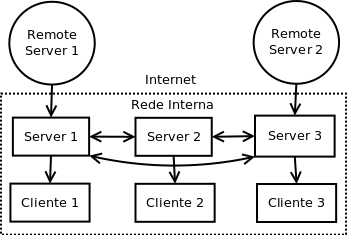
\includegraphics[scale=0.7]{image/rede_ntp_teste}
    \caption {Topologia da rede de teste.}
    \label{fig:redeNTP} 
\end{figure} 

\FloatBarrier

Têm-se, portanto, conforme a subseção anterior:

\begin{itemize}
  \renewcommand\labelitemi{--}
  \item associações cliente/servidor entre \textit{remote servers} e
  \textit{servers}, e entre \textit{servers} e \textit{clients};
  \item associações simétricas ativas entre \textit{servers}.
\end{itemize}

A fim de eliminar a necessidade de implementar essa rede fisicamente,
utilizou-se o \textit{software virtualbox}. Cada máquina presente na figura, com
exceção dos \textit{remote servers}, foi substituída por uma máquina virtual,
cujo sistema operacional é o \textit{Linux Debian 8.2.0 i386}. A escolha deste
sistema foi baseada nas características previstas para as máquinas que comporão
a infraestrutura do Sirius. Além disso, como pretende-se isolar completamente a
rede, isto é, eliminar qualquer comunicação com a Internet, os \textit{remote
servers} serão substituídos pelos respectivos servidores. Dessa maneira, tais
servidores utilizarão seus próprios relógios como fonte primária de sincronismo.

\vspace{12pt}

Foi adotado que a rede teria endereço \texttt{10.0.0.0/24}, os servidores
possuiriam endereços do tipo \texttt{10.0.0.10x}, sendo \textit{x} o dígito que
caracteriza o servidor (1, 2 ou 3), e \texttt{10.0.0.0y1} para os clientes,
sendo \textit{y} o equivalente de \textit{x}. 


\vspace{12pt}

Após a configuração de rede das respectivas máquinas virtuais, a instalação do
NTP pode prosseguir. Inicialmente, é necessário fazer a instalação do pacote
\texttt{ntp} através do comando

\begin{lstlisting}[language=bash, style=nonumbers]
$ sudo apt-get install ntp
\end{lstlisting}

Estão incluídos neste pacote, os programas \texttt{ntpd}, \texttt{ntpq}
e \texttt{ntpqc}. \texttt{ntpd}, ou \textit{NTP Daemon}, roda continuamente no
sistema e é responsável pela troca de mensagens com os diversos servidores
ou clientes, de acordo com as configurações, enquanto que \texttt{ntpq}
e \texttt{ntpqc} (o \textit{q} refere-se a \textit{query}) são utilizados para
verificar o estado das variáveis e alterar configurações do \textit{daemon}. 

\vspace{12pt}

Quando é iniciado, o \textit{daemon} retira as suas configurações do arquivo
\texttt{/etc/ntp.conf}. Cada nó da rede deve, portanto,
configurar esse arquivo de acordo com as funções que desempenha.

\vspace{12pt}

A configuração dos clientes é simples: basta adicionarmos a linha

\begin{lstlisting}[language=bash, style=nonumbers]
server 10.0.0.10y iburst
\end{lstlisting}

ao arquivo de configurações. A opção \texttt{iburst} é uma otimização fornecida
pelo protocolo que agiliza a sincronização inicial. Essa opção faz com que o
intervalo de envio de pacotes seja reduzido e a quantidade de pacotes
enviados seja aumentada caso o servidor não esteja acessível. 

\vspace{12pt}

Para o \textit{server 2}, é necessário adicionarmos as duas linhas seguintes.

\begin{lstlisting}[language=bash, style=nonumbers]
peer 10.0.0.101
peer 10.0.0.103
\end{lstlisting}

Essas duas linhas criam associações simétricas ativas entre o \textit{server 2}
e os outros servidores. Dessa maneira, eles poderão trocar informações de
sincronização entre si.

\vspace{12pt}

Para os servidores 1 e 3, além das duas linhas contendo a opção \texttt{peer}, é
necessário também adicionar as duas linhas abaixo:

\begin{lstlisting}[language=bash, style=nonumbers]
server 127.127.0.0
fudge 127.127.0.0 stratum 1
\end{lstlisting}

A primeira opção configura o relógio local do sistema como uma fonte de
sincronização, enquanto que a segunda aumenta a sua hierarquia. Se o
atributo \texttt{stratum} vale 1, logo a prioridade do respectivo servidor
torna-se máxima.

\vspace{12pt}

Para iniciar o \textit{daemon}, basta executar o comando abaixo em cada máquina.

\begin{lstlisting}[language=bash, style=nonumbers]
$ sudo /etc/init.d/ntp restart
\end{lstlisting}

Os sistemas levam alguns minutos para se sincronizarem. Para verificar o estado
das conexões e da sincronização, utiliza-se o programa \texttt{ntpq} através do
comando 

\begin{lstlisting}[language=bash, style=nonumbers]
$ ntpq -p
\end{lstlisting}

A opção \texttt{-p} lista todos os nós utilizados para sincronização do relógio
local. Para o \textit{Server 1}, espera-se uma saída parecida com a figura
\ref{fig:sv1} (não há garantias que seja idêntica, visto que os algoritmos que
determinam as fontes que serão utilizadas para sincronização são baseados em
fatores que podem variar dependendo do estado da rede). 

\FloatBarrier

\begin{figure}[h]
    
    \centering
    %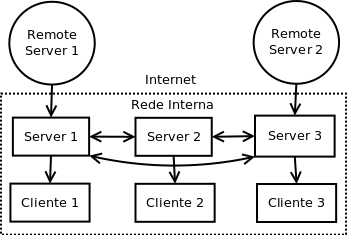
\includegraphics[scale=0.7]{image/rede_ntp_teste}
    \caption {Resultado do comando \texttt{ntpq -p} no \textit{Server 1}.}
    \label{fig:sv1} 
\end{figure} 

\FloatBarrier
\subsection {Aplicação ao projeto \textit{Sirius}}

\section {EPICS Archiver Appliance}
\label{sec:archiver}
\subsection {Introdução}

O EPICS \textit{Archiver Appliance}, desenvolvido pelo instituto americano
\textit{National Accelerator Laboratory (SLAC)}, é capaz de monitorar e arquivar
um grande número de váriaveis, geradas por servidores
EPICS presentes na rede. O sistema fornece também opções de configuração de um
largo conjunto de parâmetros referentes ao armazenamento e monitoramento. Uma
\textit{appliance} é composta basicamente por quatro módulos distintos, sendo eles:

\begin{itemize}
  \renewcommand\labelitemi{--}
  \item \textit{Management}: provê as ferramentas necessárias para a gerência
  da \textit{appliance}. Permite, por exemplo, adicionar ou remover \textit{PVs}
  à lista de variáveis a serem arquivadas;
  \item \textit{Engine}: realiza a integração entre os módulos;
  \item \textit{Data Retrieval}: módulo responsável por recuperar os dados das
  \textit{PVs} arquivadas;
  \item \textit{ETL}: responsável por extrair os dados e tranformá-los a fim de
  que as aplicações possam processá-los posteriormente;
\end{itemize}

% A figura \ref{fig:epics_archiver} esquematiza o modo de funcionamento do
% \textit{EPICS Archiver Appliance}.
% 
% \begin{figure}[h]
%     
%     \centering
%     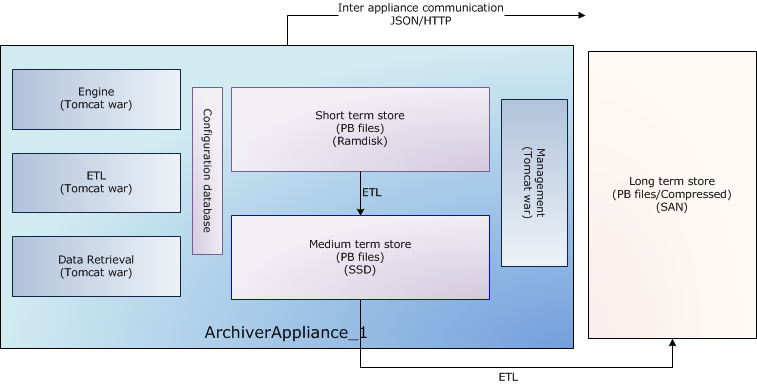
\includegraphics[scale=0.6]{image/applarch}
%     \caption {Modo de funcionamento de uma \textit{appliance}. Extraída de
%     \cite{archiver}.}
%     \label{fig:epics_archiver} 
% \end{figure} 

O instituto desenvolvedor da aplicação sugere que cada módulo seja lançado em
sua própria instância \textit{Tomcat}. Em adição, ele propõe a divisão da
unidade de armazenamento em 3 outras unidades, de acordo com a frequência em que
os dados são salvos. Essas unidades são divididas em \textit{short-term},
\textit{medium-term} e \textit{long-term storage}, cujas frequências de
armazenamento são, respectivamente, a cada hora, diária e anual. Essas
configurações podem ser modificadas através de arquivos
específicos, explicados nas próximas subseções.

\vspace{12pt}


Em um ambiente composto por diversos servidores EPICS e milhares de variáveis a
serem monitoradas, tal como o sistema de controle do \textit{Sirius}, um sistema
capaz de automatizar e agilizar o armazenamento e recuperação de dados se torna
fundamental para o monitoramento de eventuais problemas. Sendo assim, as próximas seções são
dedicadas à instalação e exploração dos recursos disponíveis nesta aplicação.

\subsection {Instalação}

A versão de Junho de 2016 do \textit{archiver} foi instalada no \textit{OPR23},
que se encontra na sala de controle, e pode ser acessada digitando-se o endereço
\texttt{10.0.4.69} em qualquer \textit{browser}. Atualmente, o arquivador possui
36 \textit{PVs} conectadas, contendo, inclusive, algumas das variáveis geradas
pelos receptores GPS, descritos na seção \ref{sec:pvsgps}. As próximas
subseções descrevem algumas das modificações realizadas no \textit{archiver}.

\subsubsection{\textit{Login} necessário}

Um dos principais problemas do arquivador é que qualquer pessoa logada
pode inserir ou remover variáveis do sistema. A fim de impedir que usuários não
autorizados realizem tais ações, modificou-se o código das
\textit{appliances} para verificar se o usuário foi autenticado com sucesso.
Para tal, instalamos um servidor LDAP no OPR23 e criamos uma página
de \textit{login}, acessada a partir de \url{http://10.0.4.69/login.html}. Quando o
usuário aperta o botão \textit{Ok}, uma requisição do tipo \textit{POST} é
enviada ao módulo \textit{PHP} que roda no servidor. Esse módulo consulta o LDAP
e retorna se o usuário foi autenticado ou não. Em caso de sucesso, uma nova
requisição do tipo \textit{POST} é enviada e capturada pelo módulo
\textit{management}, que, em seguida, inicia uma nova sessão para o usuário.
Enfim, antes de qualquer operação de inserção ou remoção de variáveis, o
módulo verifica se a sessão está definida e, caso esteja, autoriza a respectiva
operação. A intenção é integrar este sistema de \textit{login} ao servidor
LDAP do CNPEM no futuro.

\vspace{12pt}

Um usuário, denominado de \textit{Anônimo}, com permissões básicas de leitura é
disponibilizado por padrão e permite que qualquer pessoa consulte o
\textit{archiver} mesmo não estando autenticada.

\subsubsection{Mudanças no estilo}

Alguns arquivos \textit{css} (\textit{Cascading Style Sheet}) foram modificados
para refletir melhor o esquema de cores do laboratório. As imagens do
\textit{logo} também foram modificadas.

\subsection{Uso do CS-Studio no monitoramento} \label{appliance-csstudio}

O \textit{CS-Studio} \cite{css} pode ser usado para monitorar a
\textit{appliance}. Para isso, entre em \texttt{Edit \(>\) Preferences} e acesse
o item \texttt{CSS Applications \(>\) Trends \(>\) Data Browser}. No campo
\textit{Archive Data Server URLs}, adicione o endereço
\url{pbraw://10.0.4.69/lnls-control-archiver}.
Escreva qualquer \textit{Server alias}. Na tabela \textit{Default Archive Data
Sources}, adicione o mesmo endereço e aperte \textit{Ok} para salvar as
alterações.

\vspace{12pt}

É necessário alterar a perspectiva do \textit{CS Studio}. Acesse
\texttt{Windows \(>\) Open Perspective} e escolha \textbf{Data Browser}. Na aba
\textit{Archive Search}, escreva a \textit{URL} configurada anteriormente e no
campo \textit{Pattern}, escreva o nome das variáveis arquivadas que deseja
monitorar. Por exemplo, se escrevermos \texttt{Cnt:MikroE:*}, todas as variáveis
arquivadas para o receptor GPS da seção \ref{sec:pvsgps} poderão ser acessadas.
Clique com o botão direito na variável desejada e acesse \texttt{Process Variable \(>\) Data Browser}.

\subsection{Acessando a \textit{appliance} com \textit{Python}}

A \textit{appliance} pode ser acessada através de requisições \textit{JSON}
realizadas por um módulo escrito em \textit{Python}, por exemplo. Uma interface
gráfica foi implementada, usando os módulos \textit{Qt}, a fim de testarmos a
comunicação. Ela possui um gráfico, onde serão mostrados os dados recuperados,
uma caixa de opções, que possui todas as variáveis arquivadas na
\textit{appliance}, e componentes para seleção das datas de início e fim do
intervalo desejado. A figura \ref{fig:interface} representa o resultado da
implementação.

\vspace{12pt}

% \begin{lstlisting}[language=Python]
% import time
% import urllib2
% import json
% 
% class JsonRequester ():
%     
%     def __init__(self, data_retrieval_url, mgmt_url):
%         self.data_retrieval_url = data_retrieval_url
%         self.mgmt_url = mgmt_url
%     
%     def json_request_variables(self, variables_prefix):
%         
%         url_json = self.mgmt_url + 'bpl/getPVStatus?pv=' + variables_prefix
%         req = urllib2.urlopen(url_json)
%         data = json.load(req)
%         return data
%     
%     def json_request_data(self, variable, from_date, to_date):    
%         
%         retrieval_url = self.data_retrieval_url + "/data/getData.json?"
%         pv_name = ("pv=" + variable).replace(':', '%3A')
%         to_date =   ("&to=" + time.strftime("%Y-%m-%dT%H:%M:%S",to_date) + 
%         				".000Z").replace(':', '%3A')
%         from_date = ("&from=" + time.strftime("%Y-%m-%dT%H:%M:%S",from_date) + 
%         				".000Z").replace(':', '%3A')    
%         url_json = retrieval_url + pv_name + from_date + to_date
%         req = urllib2.urlopen(url_json)
%         data = json.load(req)
%         secs = [x['secs'] for x in data[0]['data']]
%         vals = [x['val'] for x in data[0]['data']]
%         return secs, vals
% \end{lstlisting}
% 
% O método construtor recebe 2 \textit{strings} como parâmetros.
% \textit{data\_retrieval\_url} e \textit{mgmt\_url} estão contidos no arquivo
% \textit{lnls\_appliances.xml} e representam, respectivamente, os endereços dos
% \textit{servlets} de obtenção de dados e gerenciamento da \textit{appliance}. A
% primeira \textit{url} será usada para recuperar os dados e a segunda, para obter
% as informações relativas às variáveis arquivadas.
% 
% \vspace{12pt}
% 
% O método \textit{json\_request\_variables} é responsável por retornar
% informações de uma ou várias variáveis, cujo nome (no caso de uma pesquisa de
% uma única variável) ou prefixo (parte comum ao nome de diversas variáveis) é
% passado como parâmetro. Para tal, utiliza o método \texttt{getPVStatus}, que é
% disponível no \textit{servlet} de gerenciamento e acessível via a \textit{url}
% \texttt{mgmt\_url}. Esse método também recebe como parâmetro nomes ou prefixos
% de variáveis, especificados após o trecho \texttt{pv=} na requisição
% \textit{json}. Para recuperar todas as variáveis arquivadas por uma
% \textit{appliance} que comecem com o prefixo \texttt{MBTemp}, por exemplo,
% bastar utilizarmos \texttt{pv=MBTemp*} na requisição. Uma vez construída a
% \textit{url}, é necessário utilizar as bibliotecas \textit{python}
% \texttt{urllib2} e \texttt{json}, que realizam a comunicação com os
% \textit{servlets}. 
% 
% \vspace{12pt}
% 
% O método \textit{json\_request\_data} retorna os dados arquivados para uma
% determinada variável, passada como parâmetro. Além dela, essa função recebe dois
% outros valores, sendo eles objetos do tipo \textit{time}, cuja implementação
% reside no módulo \texttt{time}. Esses parâmetros representam, por sua vez, as
% fronteiras do intervalo de tempo para o qual se deseja recuperar os dados, sendo
% que \texttt{from\_date} é a data mais antiga e \texttt{to\_date}, a mais
% recente. Se \texttt{to\_date} vale \texttt{None}, então o sistema o interpreta
% como o tempo no qual a chamada da função foi feita. Os dados são recuperados
% através do método \texttt{getData}, disponível no \textit{servlet}
% \texttt{retrieval} da \textit{appliance}. Antes de realizarmos a requisição, é
% necessário traduzir os objetos \textit{time} para o formato aceito pela
% servidor. Sendo assim, utiliza-se o método \texttt{strftime} do módulo
% \texttt{time} que retorna a representação \textit{string}, segundo a máscara
% especificada (no nosso caso, \texttt{\%Y-\%m-\%dT\%H:\%M:\%S}), do objeto
% passado como parâmetro. A requisição é, enfim, realizada através dos mesmos
% métodos que foram usados na função anterior.
% 
% \vspace{12pt}
% 
% O servidor envia todos os dados, isto é, valores e datas do respectivo evento,
% em único vetor de dicionários. Por este motivo, é necessário processarmos essa
% estrutura antes de retorná-la ao programa que chamou o método. Os valores são
% acessíveis pelo índice \texttt{val} e seu tipo depende da aplicação. A data dos
% eventos relativos aos valores são recuperados pelo índice \texttt{secs} e são
% números inteiros que contém o número de segundos desde uma data de referência
% (1 de Janeiro de 1970) usada no \textit{servlet}. É necessário notar que as
% datas retornadas estão em \textit{UTC}, portanto é exigido que tais
% valores sejam convertidos para a o fuso local.
% 
% \vspace{12pt}


\begin{figure}[h]
    
    \centering
    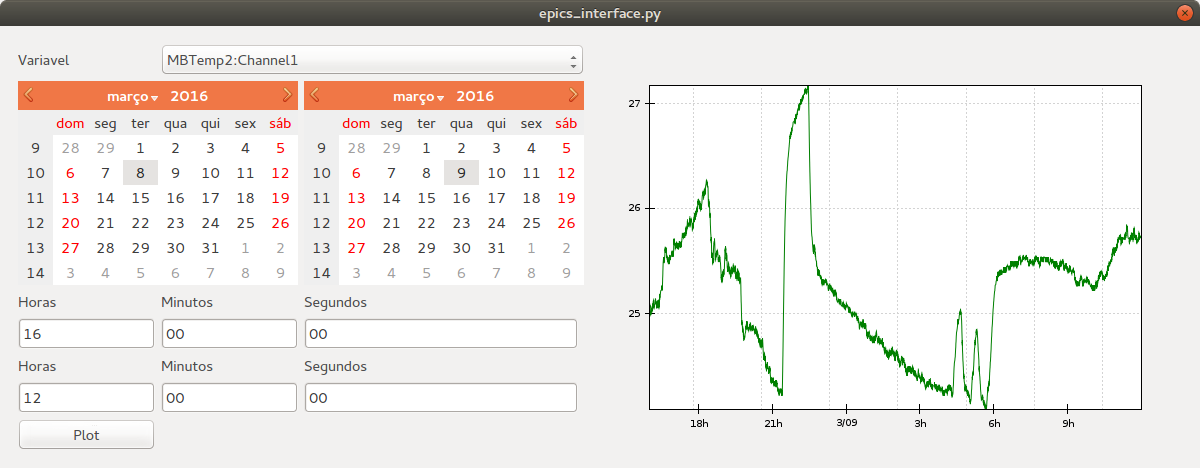
\includegraphics[scale=0.30]{image/screenshot-python}
    \caption {Interface \textit{Qt} implementada em \textit{python}.}
    \label{fig:interface} 
\end{figure} 

\section {Best Ever Alarm System Toolkit - BEAST}

\subsection {Introdução} \label{beast-intro}

Em um ambiente composto por centenas de milhares de variáveis EPICS, como o que
será implementado no \textit{Sirius}, a necessidade de um sistema capaz de
monitorar quais variáveis encontram-se em estados errôneos torna-se
imprescindível. Sendo assim, o monitor de alarmes \textit{BEAST}, do inglês
\textit{Best Ever Alarm System Toolkit} e desenvolvido pelo laboratório
americano \textit{Oak Ridge National Laboratory}, representa uma solução capaz
de gerenciar e controlar os alarmes gerados pelos servidores EPICS disponíveis
na rede. Tal sistema é implementado em \textit{Java} e é baseado no ambiente
gráfico de desenvolvimento \textit{Eclipse}. A arquitetura do sistema
está represetada na figura \ref{fig:best_arquitetura}, logo abaixo.

\FloatBarrier

\begin{figure}[h]

\centering
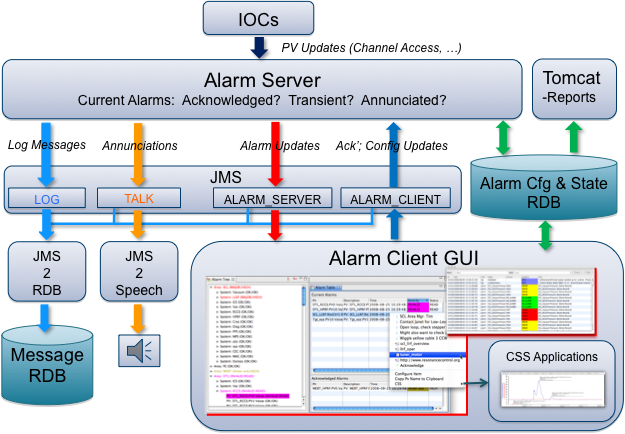
\includegraphics[scale=0.55]{image/beast-arquitetura}
\caption {Implementação do sistema de monitoramento de alarmes
\textit{BEAST}.}
\label{fig:best_arquitetura}
\end{figure}

\FloatBarrier

É possível distinguir diversos componentes na figura acima:

\begin{enumerate}[i.]
  
  \item \textit{Alarm server}: o servidor é responsável por tarefas fundamentais
  no monitoramento de alarmes. Cabe a ele a leitura da configuração dos alarmes
  armazenada no banco de dados \textit{Alarm Cfg \& State RDB}, conectar-se às
  respectivas variávies, monitorar suas mudanças de estado e gerar alarmes
  quando necessário e desativá-los logo que um operador toma conhecimento
  do problema. Esse módulo permite que um número variável de clientes se conecte
  a ele. Uma variável pode adotar duas configurações distintas, sendo elas
  \textit{latch} e \textit{annunciate}. Para a primeira, o servidor mantém o
  alarme de maior gravidade, mesmo que o estado da variável não seja
  atualmente errôneo, até que ele seja reconhecido manualmente pelo operador.
  A fim de impedir um grande volume de alarmes gerados, é possível habilitar
  as opções \textit{delay}, que aciona o alarme somente se o estado errôneo da
  variável se mantiver durante o intervalo de tempo especificado, e
  \textit{count}, que aciona o alarme se tal estado for detectado mais vezes
  que o valor especificado. A segunda configuração ativa o alarme somente
  quando a \textit{PV} apresentar valor inválido, sendo que ele é desativado
  logo que tal variável voltar à sua faixa de operação esperada.
  
  \item \textit{Alarm Cfg \& State RDB}: banco de dados relacional, como um
  servidor \textit{MySQL} por exemplo, onde serão armazenadas as configurações
  de alarme e o atual estado de todos os alarmes.
  
  \item \textit{Java Message Service - JMS}: utilizado para a comunicação entre
  diferentes módulos. No projeto, foi empregada a implementação realizada pelo
  \textit{Apache Software Foundation} chamada de  \textit{Apache ActiveMQ}. O
  sistema utiliza 4 \textit{topics} distintos, sendo eles:
  
  \begin{itemize} \renewcommand\labelitemi{--}
    \item \textit{ALARM\_SERVER}: utilizado pelo servidor para publicar
    atualizações nos estados dos alarmes de acordo com a configuração de cada
    variável.
    
    \item \textit{ALARM\_CLIENT}: permite que clientes notifiquem atualizações
    de configuração e reconhecimento de alarmes.
    
    \item \textit{TALK}: dedicado para anunciar mensagens.
    
  \end{itemize}
  
  \item \textit{Alarm Client GUI}: \label{client-gui} baseado na interface
  gráfica do \textit{Eclipse}, oferece três opções de monitoramento:
  
  \begin{itemize} \renewcommand\labelitemi{--}
    \item \textit{Alarm table}: mostra os alarmes em duas tabelas distintas
    contendo aqueles reconhecidos (\textit{acknowledged alarms}) e aqueles que
    ainda estão acionados (\textit{active alarms}).
    
    \item \textit{Alarm tree}: essa opção de visualização oferece
    uma visão hierarquica dos alarmes, sendo organizada, do nível mais alto para
    o menor, em áreas, sistemas, subsistemas e variáveis. Oferece opções para
    configurar, remover ou adicionar variáveis no nível desejado. O estado do
    alarme de cada item é mostrado por uma cor e por uma anotação, sendo
    composta por três sentenças entre parênteses, que representam
    respectivamente a gravidade atual (\textit{current severity}), a
    maior gravidade detectada anteriormente (\textit{alarm severity}) e o estado
    atual do alarme (\textit{alarm status}). É sincronizada diretamente ao banco
    \textit{Alarm Cfg \& State RDB}, o que implica que uma mudança realizada é
    rapidamente detectada pelo servidor e pelos demais clientes.
    
    \item \textit{Alarm area panel}: indicação gráfica do estado do sistema.
    
  \end{itemize}
  
  É possível, a partir de qualquer uma das \textit{views} presentadas acima,
  acessar outros recursos, como, por exemplo, gráficos e valores atuais das
  variáveis desejadas. Para isso, basta apertar com o botão direito acima da
  \textit{PV} e apertar em \textit{Process variables}.
  
  \vspace{12pt}
  
  A implementação fornece, ainda, suporte para autenticação de usuários via
  \textit{LDAP} ou \textit{JAAS}. Caso seja a escolha, somente usuários
  autorizados podem alterar as configurações de alarmes ou reconhecê-los.
  
  \item \textit{Web reports}: é fornecido também um conteúdo \textit{Web} capaz
  de gerar relatórios, calcular estatísticas (como, por exemplo, totais
  diários, variáveis que mais disparam alarmes, intervalos de tempo que os
  alarmes permanecem mais ativos em média \textit{etc.}) e monitorar os alarmes.
  Assim como os módulos do \textit{EPICS Archiver Appliance}, as páginas devem estar hospedadas em um
  servidor \textit{Tomcat}.
  
\end{enumerate}

\subsection{Instalação}

\textit{BEAST} necessita de uma base de dados relacional, de uma implementação
\textit{JMS} e de um ambiente gráfico baseado no \textit{Eclipse}. Utilizaremos,
respectivamente, o \textit{MySQL}, \textit{Apache ActiveMQ} e a versão
\textit{Eclipse Luna for RCP and Plugin Development}. Uma sugestão de instalação
é apresentada abaixo.

\begin{enumerate}[i.]
  \item  É necessário inicialmente fazer o \textit{download} do
  código fonte do \textit{CS Studio} para obter o produto relacionado ao \textit{Alarm server}.
  Para isso, acesse o repositório do projeto no \textit{GitHub} e extraia os
  arquivos em um diretório. Usaremos aqui o mesmo caminho especificado por
  \texttt{\$INSTALL\_DIR}, utilizado também na seção \ref{sec:archiver}.
  
  \begin{lstlisting}[keywordstyle=\ttfamily, style=nonumbers]
$ cd $INSTALL_DIR/
$ wget https://github.com/ControlSystemStudio/cs-studio/archive/master.zip
$ unzip cs-studio-master.zip
$ rm cs-studio-master.zip
$ cd cs-studio-master/
\end{lstlisting}
   
   Na pasta \texttt{cs-studio-master/}, estão contidos todos os arquivos com os
   códigos-fonte do \textit{CS Studio}, porém só utilizaremos o diretório \texttt{applications/},
   que é o onde está a implementação do \textit{Alarm server}.
   
   \item \label{mysql-alarm} Antes de executar o servidor, é necessário primeiro
   configurar o banco de dados com as tabelas utilizadas por ele. Para isso, diversos
   \textit{scripts} de instalação são disponibilizados pelo desenvolvedor em 
   \texttt{applications/alarm/alarm-plugins/org.csstudio.alarm.beast/dbd}. Vamos
   usar parte do conteúdo contido em \texttt{ALARM\_MYSQL.sql}, uma vez que
   este arquivo adiciona algumas entradas nas tabelas, a fim de testar a
   aplicação. Abra este arquivo e comente as linhas a partir de \texttt{INSERT
   INTO ALARM.ALARM\_TREE VALUES (3, 2, 'System', now());}. As linhas acima
   desta sentença criam a hierarquia, que também nos será útil. Execute, então,
   os seguintes comandos:
   
\begin{lstlisting}[basicstyle=\fontsize{9}{13}\selectfont\ttfamily,
keywordstyle=\ttfamily, style=nonumbers] $ mysql -u root -p
>> CREATE DATABASE ALARM;
>> GRANT ALL ON ALARM.* TO 'lnls_alarm_user'@localhost IDENTIFIED BY 'alarm_password';
>> exit
$ mysql -u lnls_alarm_user -p
>> source applications/alarm/alarm-plugins/org.csstudio.alarm.beast/dbd/ALARM_MYSQL.sql;
\end{lstlisting}

Verifique que as tabelas foram criadas corretamente com:

\begin{lstlisting}[keywordstyle=\ttfamily, style=nonumbers]
>> SHOW TABLES;
\end{lstlisting}
   
\item A próxima etapa é configurar o servidor de mensagens \textit{JMS}. Será
necessário fazer o \textit{download} do pacote \textit{Apache ActiveMQ}.

\begin{lstlisting}[keywordstyle=\ttfamily, style=nonumbers]
$ cd $INSTALL_DIR/
$ wget http://tinyurl.com/htw5tdx
$ tar -xvzf apache-activemq-5.13.0-bin.tar.gz
$ rm apache-activemq-5.13.0-bin.tar.gz
$ cd apache-activemq-5.13.0/
\end{lstlisting}

O diretório \texttt{conf/} contem um arquivo, \texttt{activemq.xml}, com as
configurações do servidor. É possível, por exemplo, modificar a porta, que por
padrão é 61616, ou adicionar autenticação via \textit{jaas}. Para tal, adicione
as seguintes linhas neste arquivo.

\begin{lstlisting}[keywordstyle=\ttfamily, style=nonumbers]
<plugins>
  <jaasAuthenticationPlugin configuration="PropertiesLogin" />
</plugins>
\end{lstlisting}

Neste caso, \textit{PropertiesLogin} é o nome da configuração contido no arquivo
\texttt{login.config}, que especifica os \textit{plugins} necessários e os
arquivos onde estarão armazenados os usuários, suas senhas (\texttt{users.properties}) e grupos
(\texttt{groups.properties}). Por fim, inicie o servidor com 

\begin{lstlisting}[keywordstyle=\ttfamily, style=nonumbers]
$ cd $INSTALL_DIR/apache-activemq-5.13.0/bin/linux-x86-64/
$ ./activemq start
\end{lstlisting}

\item Tendo instalado os componentes responsáveis pela comunicação entre módulos
e base de dados de configurações, podemos iniciar o servidor. Para isso, vamos
utilizar a distribuição \textit{Luna} do \textit{Eclipse for RCP and RAP
Developers}, por apresentar melhor compatibilidade com os pacotes gráficos do
\textit{CS Studio}. Extraia e inicie a aplicação.

\begin{lstlisting}[keywordstyle=\ttfamily, style=nonumbers]
$ cd $INSTALL_DIR/
$ wget http://tinyurl.com/jbmmue7
$ tar -xvzf eclipse-rcp-luna-SR2-linux-gtk-x86_64.tar.gz
$ rm eclipse-rcp-luna-SR2-linux-gtk-x86_64.tar.gz
$ cd eclipse/
$ ./eclipse
\end{lstlisting}

Importe o projeto que contem o servidor de alarmes. Para tal, entre em
\texttt{File > Import \ldots > General > Existing Projects into Workspace} e
escolha o diretório \texttt{\$INSTALL\_DIR/ applications/alarm/}. Dentro deste
projeto, abra o arquivo \texttt{AlamServer.product} contido em
\texttt{alarm-plugins > org.csstudio.alarm.beast.server}. Espera-se que uma tela
parecida com a figura \ref{img:product-view} seja aberta.

\FloatBarrier

\begin{figure}[h]

\centering
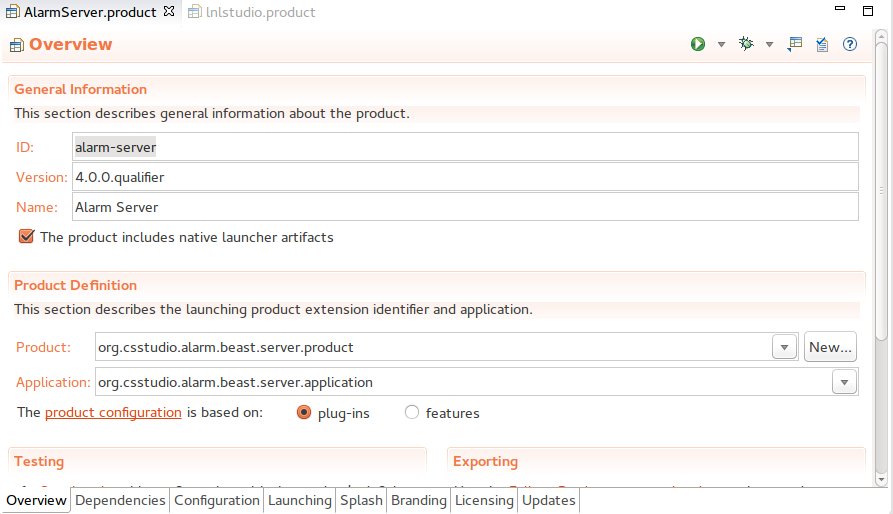
\includegraphics[scale=0.45]{image/product-view}
\caption {Configurações do produto \texttt{AlarmServer.product}.}
\label{img:product-view} 
\end{figure}

\FloatBarrier

Ainda não é possível executá-la, visto que este produto requer algumas
depedências. Para incluí-las à instalação do \textit{Eclipse}, acesse
\texttt{Help > Install New Software\ldots > Add\ldots} e adicione a \textit{url}
\textit{http://download.controlsystemstudio.org/updates/4.1}. Não é necessário
realizar o \textit{download} de todos os pacotes, somente os espeficados na
tabela \ref{tab:plugins} abaixo. A instalação também adiciona os componentes que
permitem o acesso à \textit{appliance}, conforme explicado na seção
\ref{appliance-csstudio}. 

\FloatBarrier
\begin{longtable}[h] {| p{0.3\linewidth} | p{0.3\linewidth} | p{0.3\linewidth}   |}
\caption{\label{tab:plugins} \textit{Plugins} necessários para o
\textit{AlarmServer}.}\\
\hline \multicolumn{3}{| c |}{\textbf{CS-Studio Applications}} \\ \hline
\hline Alarm Handler Tools & Alarm Handler UI & Appliance Archiver Reader (x2) \\ \hline
Application Utilities & Archive Reader RDB Feature & Archive Tools Feature \\ \hline
CS-Studio Epics v3 Support & CS-Studio RAP Utilities & Data Browser \\ \hline
Data Browser OPI Widget & ea4 Archiver Reader & Operator Interface Builder (BOY)\\
\hline \hline \multicolumn{3}{| c|}{\textbf{CS-Studio Core}} \\ \hline \hline
Core Auth Feature & Core Base Feature & Core Platform plugins   \\ \hline
Core Platform RAP Plugins & Core UI Feature & Core Utility Feature \\ \hline
CS-Studio Command-line Execution Services Support & CS-Studio Common Data
Layer (pvmanager) & CS-Studio DAL \\ \hline
CS-Studio Epics v4 Support & CS-Studio Extras Support & PVManager
Autocomplete Featue \\ \hline \hline
\multicolumn{3}{| c|}{\textbf{Maven osgi-bundles}}  \\ \hline \hline
antlr & EPICS Plug-in & Graphene \\ \hline
JSON support for file datasource & JSR 353 API & JSR 353 Default Provider \\ \hline
org.antlr.runtile & org.epics.graphne & org.epics.util \\\hline
org.epics.vtype & org.epics.vtype-json &  org.python.jython \\\hline
pvAccess - Java & pvData - Java &  PVManager Core \\\hline
PVManager EPICS Channel Access Support  & PVManager EPICS PVAccess Support  & 
PVManager Execute Support \\\hline
PVManager File Support  & PVManager Local PV Support  & 
PVManager Simulated PV Support \\\hline
PVManager System Support  & PVManager VType Support  & \\\hline
\end{longtable}
\FloatBarrier

O produto necessita também do \textit{plug-in} \texttt{com.ibm.icu.base} contido
no repositório \textit{Orbit}, acessado através do \textit{link} abaixo.
Selecione somente o pacote \textit{Internacional Components for Unicode for
Java (ICU4J)} e instale-o.

\begin{center}
\textit{http://download.eclipse.org/tools/orbit/downloads/drops/R20150124073747/repository/}
\end{center}

O servidor já pode ser executado, porém ele utilizará uma configuração padrão
para conectar-se ao \textit{MySQL} e ao \textit{JMS}. A fim de modificar tal
configuração, editamos o arquivo \textit{plugin\_ customization.xml}, presente
no mesmo diretório. Esse arquivo deve refletir as instalações realizadas
anteriormente. 

\vspace{12pt}

Entre na aba \texttt{Launching} e adicione o argumento
\texttt{-pluginCustomization} no campo \textit{Program Arguments}. Tal argumento
deve conter o caminho do arquivo \textit{plugin\_customization.xml}, conforme
figura abaixo.

\FloatBarrier

\begin{figure}[h]

\centering
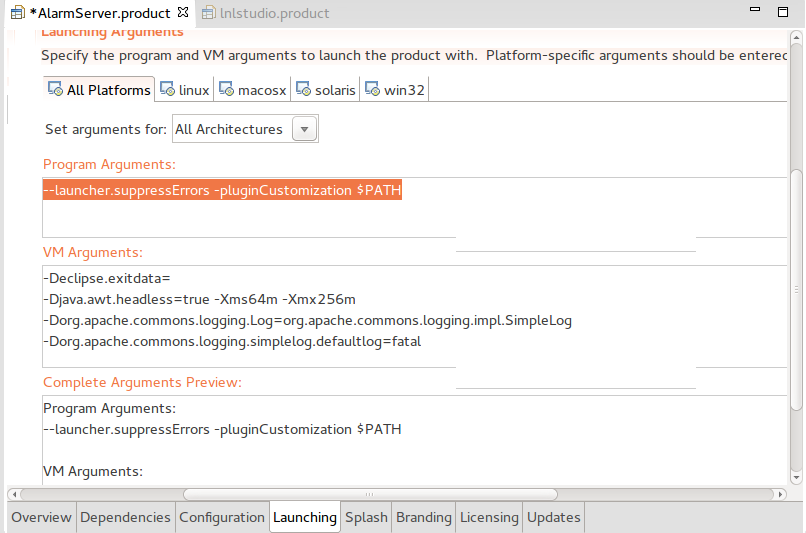
\includegraphics[scale=0.45]{image/launch-view}
\caption {\textit{Launching view} do produto \texttt{AlarmServer.product}.
Substituir \texttt{\$PATH\_TO\_FILE}} pelo caminho completo do arquivo
\textit{plugin\_customization.xml}.
\label{img:launch-view} 
\end{figure}

\FloatBarrier

Execute, enfim, o produto apertando no ícone verde no canto superior direito.
O servidor se encarregará da criação dos \textit{topics} na aplicação
\textit{JMS}. O resultado esperado está representado na figura
\ref{fig:server-on}. \textit{Annunciator} é o nome dado à raíz da hierarquia
criada no item \ref{mysql-alarm} (verificar conteúdo do arquivo
\texttt{ALARM\_MYSQL.sql}) e define, assim, quais tópicos serão utilizados na
comunicação.

\FloatBarrier

\begin{figure}[h]

\centering
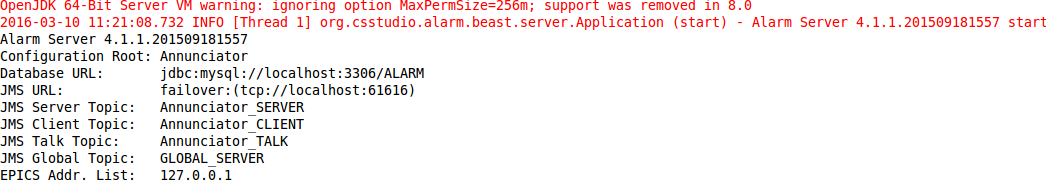
\includegraphics[scale=0.45]{image/alarmserver-on}
\caption {Resultado da execução do produto \textit{AlarmServer}.}
\label{fig:server-on} 
\end{figure}

\FloatBarrier

\end{enumerate}

\subsection{Uso da interface \textit{Eclipse} como \textit{Alarm Client GUI}}

Para configurar o \textit{Eclipse} como um cliente do servidor de alarmes, é
necessário configurá-lo para que ele acesse os servidores \textit{MySQL} e
\textit{JMS}. Isso é realizado através de \texttt{Window > Preferences > CSS
Applications > Alarm > Alarm System}. Modifique os campos\footnote{\textit{RDB}
significa \textit{Relational Database}, como o banco de dados \textit{MySQL}.}
\textit{url}, \textit{username} e \textit{password}, conforme configurado
anteriormente, e reinicie o \textit{Eclipse}. Se tudo foi configurado
corretamente, já é possível acessar os alarmes configurados através do
componentes comentados no item \ref{client-gui} da seção \ref{beast-intro}. Tais
componentes são acessados a partir de \texttt{Window > Show View > Other > CSS}.


\subsubsection {\textit{Debugging}} 

Alguns erros foram encontrados durante a instalação:

\begin{enumerate}[i.]
  \item \textit{A interface não salva corretamente as senhas do banco de dados e
  do JMS}: para resolver este problema basta redefir as senhas que o
  \textit{Eclipse} utiliza para criptografar as senhas salvas. Acesse
  \texttt{Window > Preferences > General > Security > Secure Storage} e redefina
  as senhas contidas na tabela \textit{Master password providers}.

  \item \textit{Não é possível adicionar, remover ou configurar variáveis a
  partir da Alarm Tree View}: conforme explicado na seção \textbf{Introdução}, o
  \textit{BEAST} oferece suporte à autenticação e autorização de usuários. Sendo
  assim, somente usuários cadastrados são permitidos de alterar ou reconhecer
  alarmes. Como a rede do \textit{Sirius} é prevista para ser isolada, tal
  serviço não será necessário. Portanto, podemos configurar o \textit{Eclipse}
  para dar permissão completa a qualquer \textit{user}. Para tal, devemos
  modificar o plugin \texttt{org.csstudio.security}, de extensão \textit{.jar}
  presente no diretório \textit {\$INSTALL\_DIR/eclipse/plugin}. Abra esse
  arquivo com o \textit{Archive Manager} (em sistemas \textit{linux}),
  modifique o campo \texttt{alarm\_config} para \texttt{.*} no arquivo
  \texttt{authorization.conf} e reinicie o \textit{Eclipse}. Deve ser possível
  alterar configurações de alarmes a partir de agora.
\end{enumerate}

\subsubsection {Obtendo um \textit{LNLStudio} a partir da configuração do
\textit{Eclipse}}

É possível exportar a configuração atual do \textit{Eclipse} como um novo
produto, que chamaremos de \textit{LNLStudio}. Para isso, criamos um novo um
novo \textit{Plug-in Project} e adicionamos um novo arquivo do tipo
\textit{Product Configuration}. Neste arquivo, definimos nome, \textit{id},
versão e, no campo \textit{Product Definition}, definimos \textit{Product} como
\texttt{lnlstudio.product} e \textit{Application},
\path{org.eclipse.ui.ide.workbench}. Na aba \textit{Dependencies}, é preciso
especificar quais \textit{plug-ins} são necessários ao produto. Por questão de
simplicidade, adicionamos todos aqueles que estão instalados
(\textit{Add\ldots} e \textit{Ctrl+A} para selecionar todos). Para configurar a
\textit{splash screen}, clique na aba \textit{Splash} e adicione uma
\textit{progress bar}, uma \textit{progress message} e um arquivo chamado
\textit{splash.bmp} ao diretório do projeto. Essa imagem deve possuir dimensões
455x295. 

\vspace{12pt}

O produto pode ser lançado através do ícone verde presente no canto superior da
tela.

\vspace{12pt}

Para exportar este produto, clique em \textit{Eclipse Product export wizard} na
seção \textit{Exporting} da aba \textit{Overview} e escolha o endereço e formato
(arquivo \textit{.zip} ou pasta) para o qual ele deve ser exportado. Para
executar, entre na pasta criada (ou extraída do arquivo) e execute o aplicativo
\texttt{eclipse}.


\section* {Referências bibliográficas}
\begin {itemize}
  \item \url{https://en.wikipedia.org/wiki/Sunspot}. Acessado às 19:22 29/09/2015.
  \item Guyon, I.; Elisseeff, A. "An introduction to variable and feature selection", Journal of Machine Learning Resear ch, vol. 3, pp. 1157 - 1182 2003.
  \item \url{http://archive.ics.uci.edu/ml/datasets/Wine+Quality}.\\
  	 Acessado às 21:27 30/09/2015.
\end{itemize} 
    

\end{document}
